\documentclass{article}
\usepackage{graphicx}
\usepackage{media9}
\usepackage{animate}

\begin{document}
See here.

%\includemedia[width=.8\linewidth,height=0.8\linewidth,3Dmenu,activate=pageopen,
%3Droll=-26.20348116580949,
%3Dc2c=0.2903803884983063 0.8651841282844543 -0.4088222086429596,
%3Dcoo=0.003452301025390625 0.001689910888671875 85.78641510009766,
%3Droo=577.9480034506856,
%3Dlights=Headlamp,add3Djscript=asylabels.js]{
\includegraphics{text_example}}{text_example.prc}

%\includemedia[width=.8\linewidth,activate=pageopen]{}{3Danimationtest}

\begin{tabular}{c}
{\includemedia[width=.8\linewidth,height=0.8\linewidth,3Dmenu,activate=onclick,
3Droll=0,
3Dc2c=0 0 1,
3Dcoo=4 4 2,
3Droo=159.05549293569894,
3Dortho=0.004,
3Dlights=Headlamp,add3Djscript=asylabels.js]{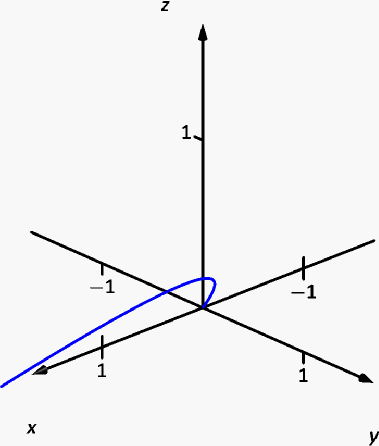
\includegraphics{surface_test}}{surface_test.prc}}\\
(a)\\
\end{tabular}




\end{document}
